\documentclass[a4paper,12pt]{report}
\usepackage[T1]{fontenc}
\usepackage[utf8]{inputenc}
\usepackage[italian]{babel}
\usepackage{graphicx} % Per le immagini
\usepackage{enumitem} % Liste numerate
\usepackage{tabularx} % Per tabelle
\usepackage{booktabs} % Per tabelle
\usepackage{float} % Per bloccare le immagini
\usepackage{url}
\usepackage{longtable}
\usepackage{dirtree}
\usepackage{pgfgantt} % strumento per generare GANTT

\title{Manuale Utente \\ \large Wiki Collaborativo per Appunti}
\author{Domenico Aloi}
\date{Anno Accademico 2025/26 - Ingegneria del Software}

\begin{document}

\maketitle

\chapter{Introduzione}
\noindent Il sistema \textit{Wiki Collaborativo} è una piattaforma web progettata per la condivisione e il versionamento di appunti universitari. L'interfaccia è di tipo \textit{Single Page Application}, garantendo una navigazione rapida tra i contenuti senza ricaricamenti della pagina.

\begin{figure}[H]
    \centering
    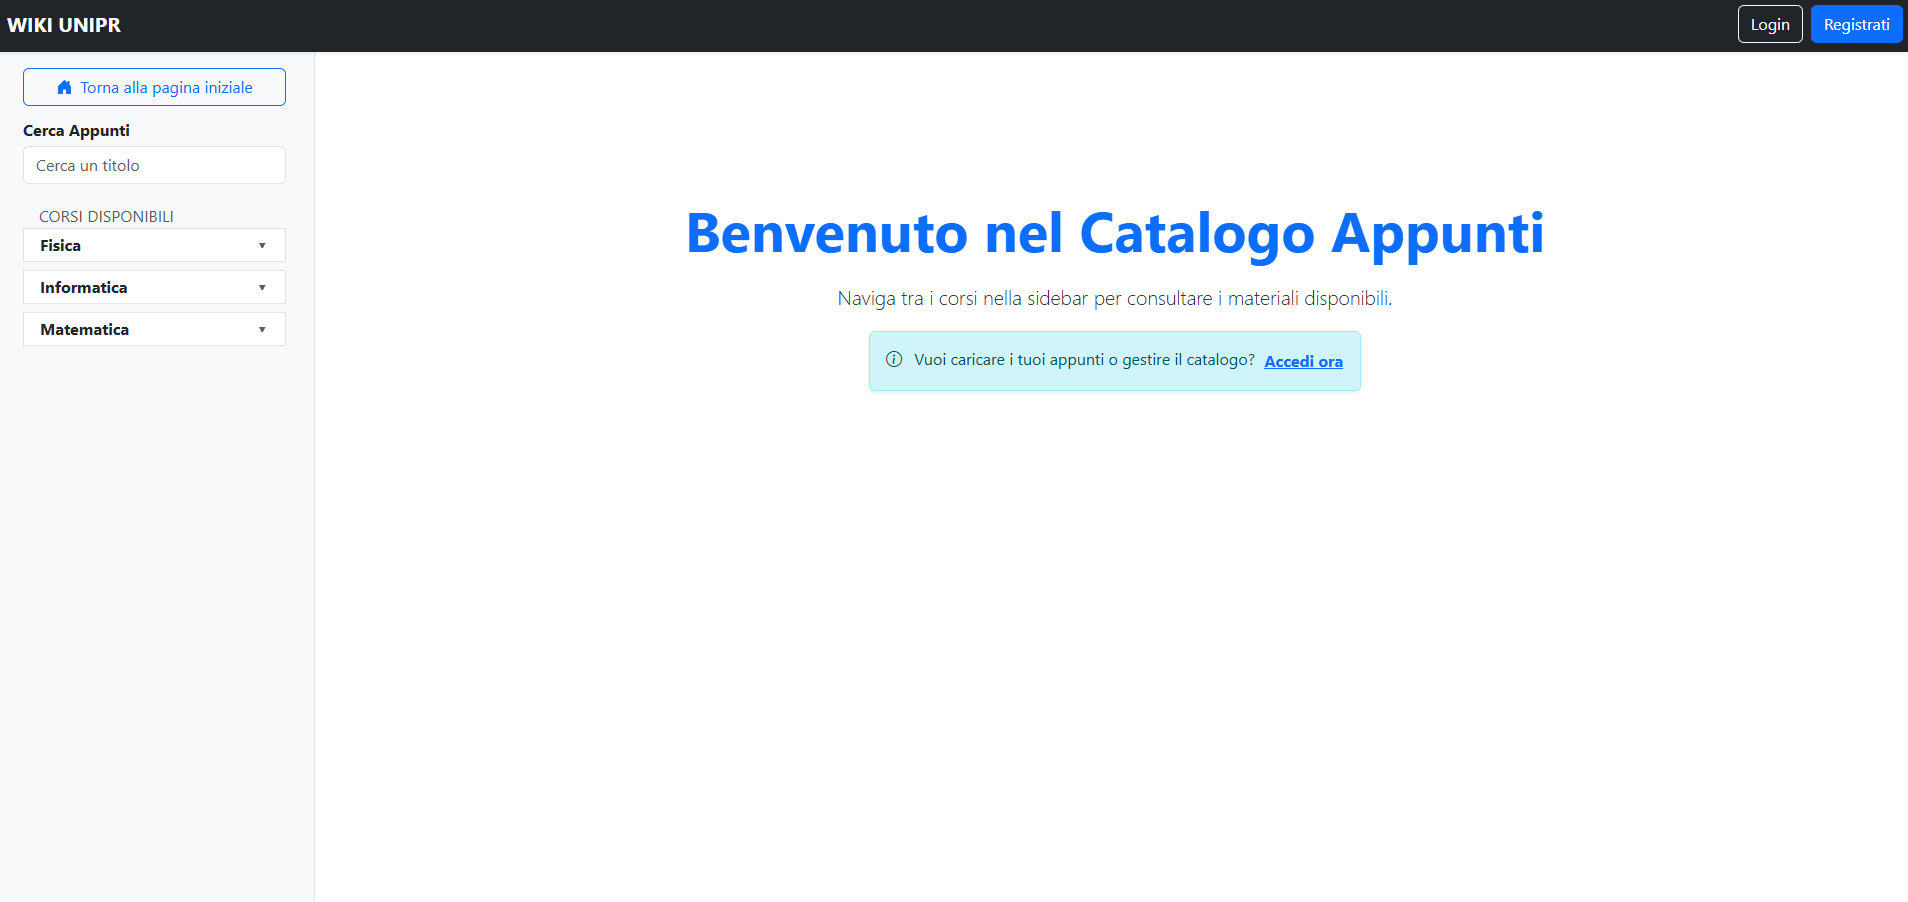
\includegraphics[width=1\textwidth]{Screen/UNO.png}
    \caption{Pagina iniziale}
    \label{fig:Home}
\end{figure}

\chapter{Modalità visitatore}

\section{Accesso e Registrazione}
\begin{itemize}
    \item \textbf{Registrazione} Figura~\ref{fig:registrazione}: I nuovi utenti possono creare un account tramite l'apposito modulo, fornendo un'email valida e una password.
    \item \textbf{Login} Figura~\ref{fig:login}: L'accesso abilita le funzionalità di scrittura e gestione della cronologia. Gli utenti non autenticati (\textit{Visitatori}) possono comunque consultare e cercare tutti i contenuti.
\end{itemize}

\begin{figure}[H]
    \centering
    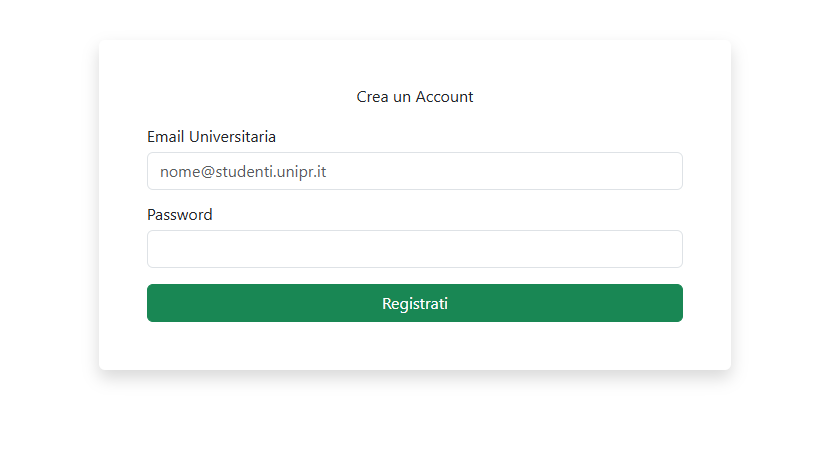
\includegraphics[width=0.8\textwidth]{Screen/registrazione.png}
    \caption{Registrazione}
    \label{fig:registrazione}
\end{figure}

\begin{figure}[H]
    \centering
    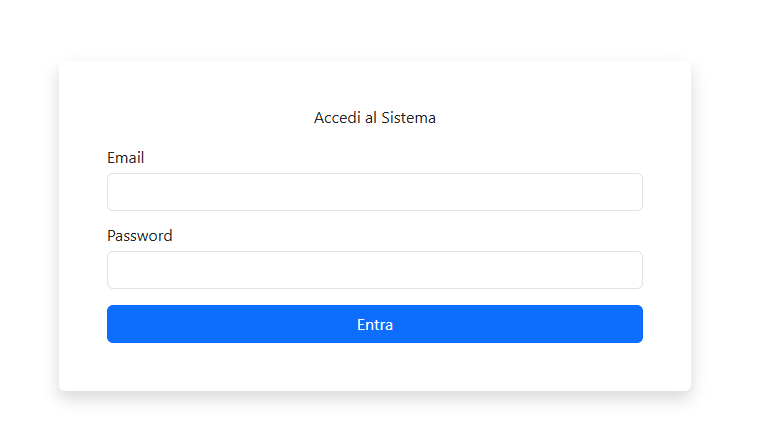
\includegraphics[width=0.8\textwidth]{Screen/login.png}
    \caption{Login}
    \label{fig:login}
\end{figure}


\section{Navigazione e Consultazione}
\noindent La navigazione si articola su tre livelli gerarchici:
\begin{enumerate}
    \item \textbf{Selezione Corso} (Figura~\ref{fig:sidebar}): Dalla barra laterale o dalla home è possibile scegliere il corso di interesse (es. Informatica).
    \item \textbf{Selezione Argomento} (Figura~\ref{fig:sidebar}): Una volta scelto il corso, verranno visualizzati i relativi argomenti (es. Meccanica).
    \item \textbf{Lettura Appunto} (Figura~\ref{fig:appunti_argomento} e Figura~\ref{fig:appunto_visualizza}) : Selezionando un appunto, il contenuto verrà renderizzato in formato HTML a partire dal sorgente Markdown.
    \item \textbf{Ricerca}: Tramite la barra di ricerca, è possibile individuare rapidamente gli appunti inserendo almeno due caratteri del titolo.
\end{enumerate}

\begin{figure}[H]
    \centering
    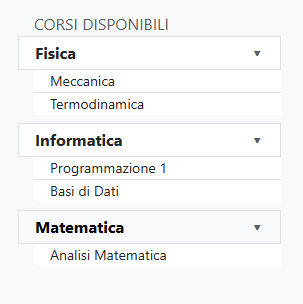
\includegraphics[width=0.5\textwidth]{Screen/sidebar.png}
    \caption{Sidebar aperta che mostra corsi e argomenti}
    \label{fig:sidebar}
\end{figure}

\begin{figure}[H]
    \centering
    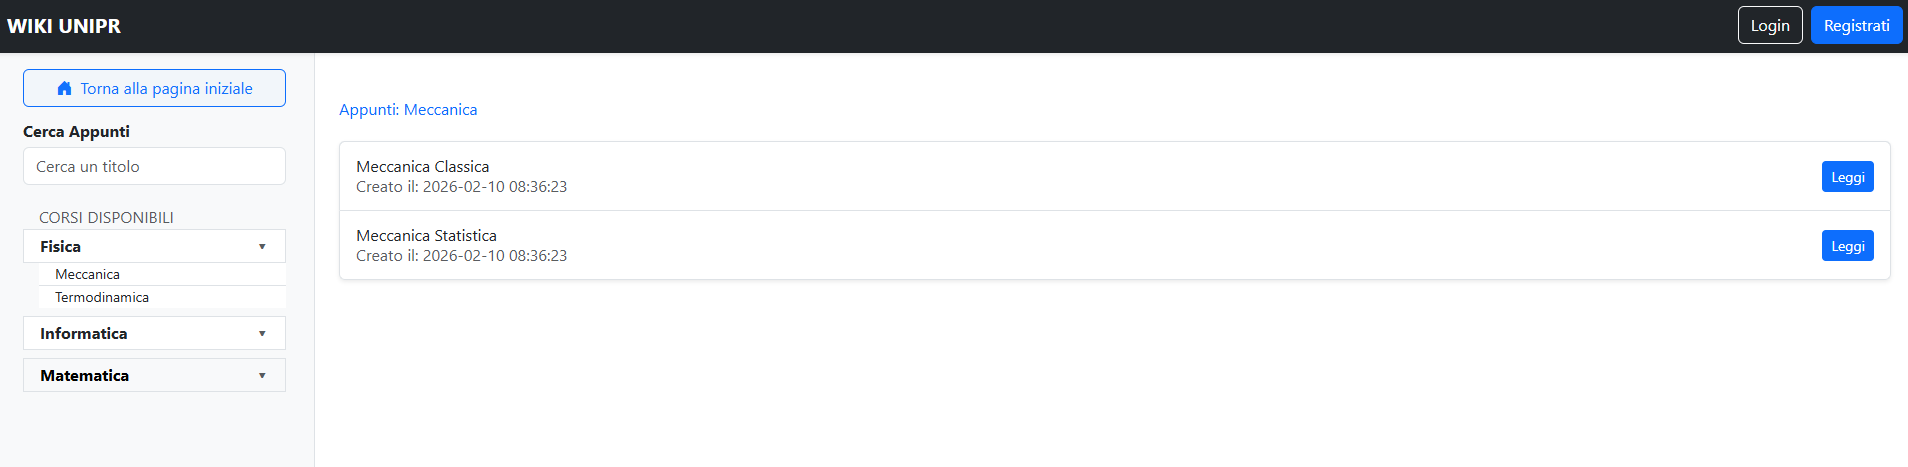
\includegraphics[width=1\textwidth]{Screen/appunti_argomento.png}
    \caption{Elenco appunti per argomento}
    \label{fig:appunti_argomento}
\end{figure}

\begin{figure}[H]
    \centering
    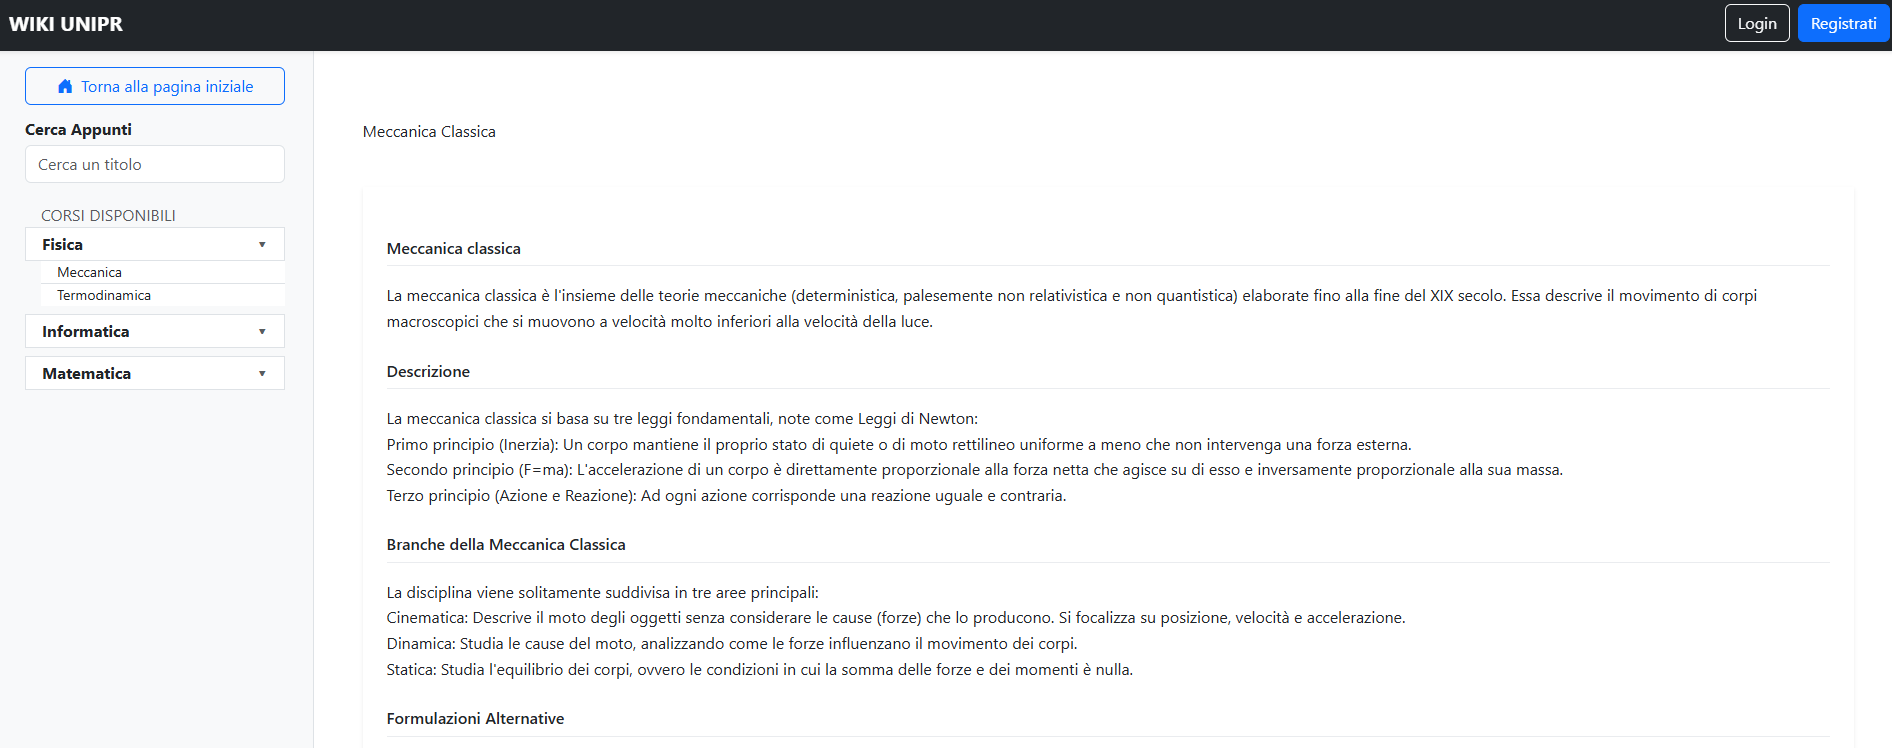
\includegraphics[width=1\textwidth]{Screen/appunto_visualizza.png}
    \caption{Appunto in modalità visitatore}
    \label{fig:appunto_visualizza}
\end{figure}

\chapter{Modalità Studente}

\section{Gestione degli Appunti (Solo Studenti)}
\noindent Gli utenti autenticati con ruolo \texttt{studente} hanno accesso alle seguenti funzioni:
\begin{itemize}
    \item \textbf{Creazione}: Utilizzando il pulsante \textit{``+ Crea Nuovo Appunto''} (Figura~\ref{fig:appunti_argomento_logged}), si apre la sezione in cui l'utente può inserire un titolo e il testo (Figura~\ref{fig:crea_appunto}) (supporta la sintassi Markdown).
    \item \textbf{Modifica}: Aprendo un appunto esistente, è possibile modificarne il contenuto (Figura~\ref{fig:appunto_logged}). Ogni salvataggio genera automaticamente una nuova versione.
\end{itemize}

\begin{figure}[H]
    \centering
    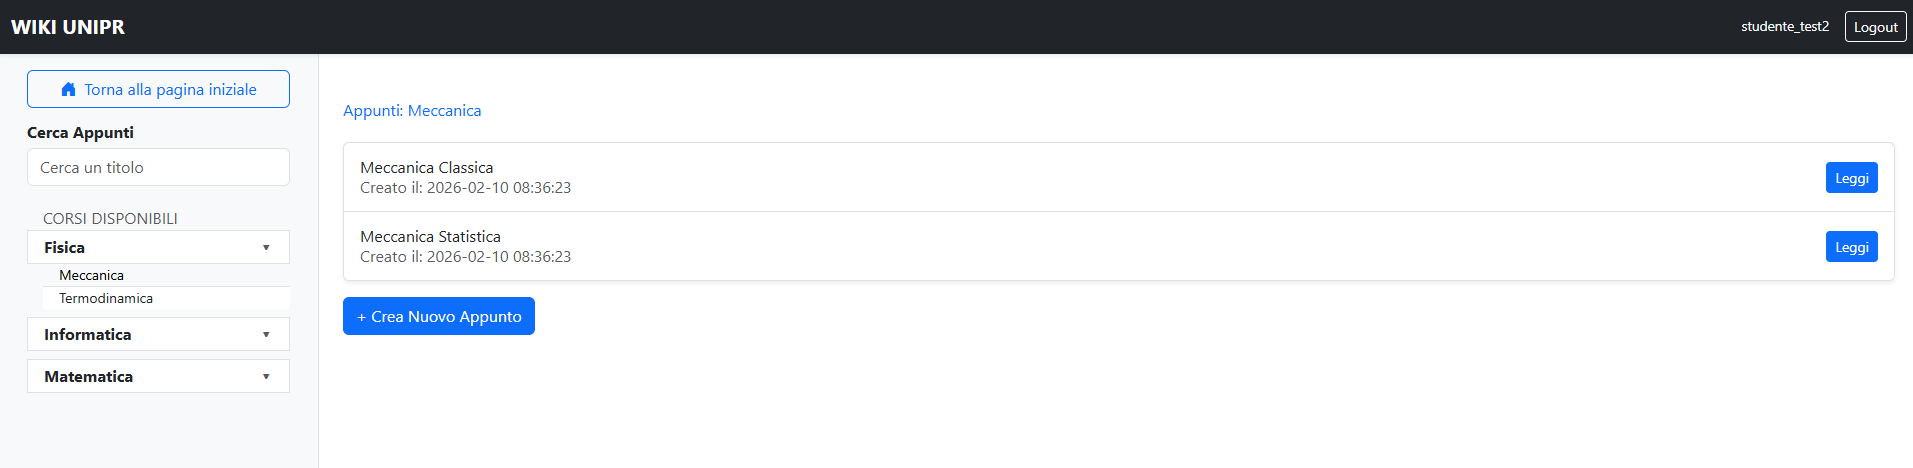
\includegraphics[width=1\textwidth]{Screen/appunti_argomento_logged.png}
    \caption{Elenco appunti per argomento modalità studente}
    \label{fig:appunti_argomento_logged}
\end{figure}

\begin{figure}[H]
    \centering
    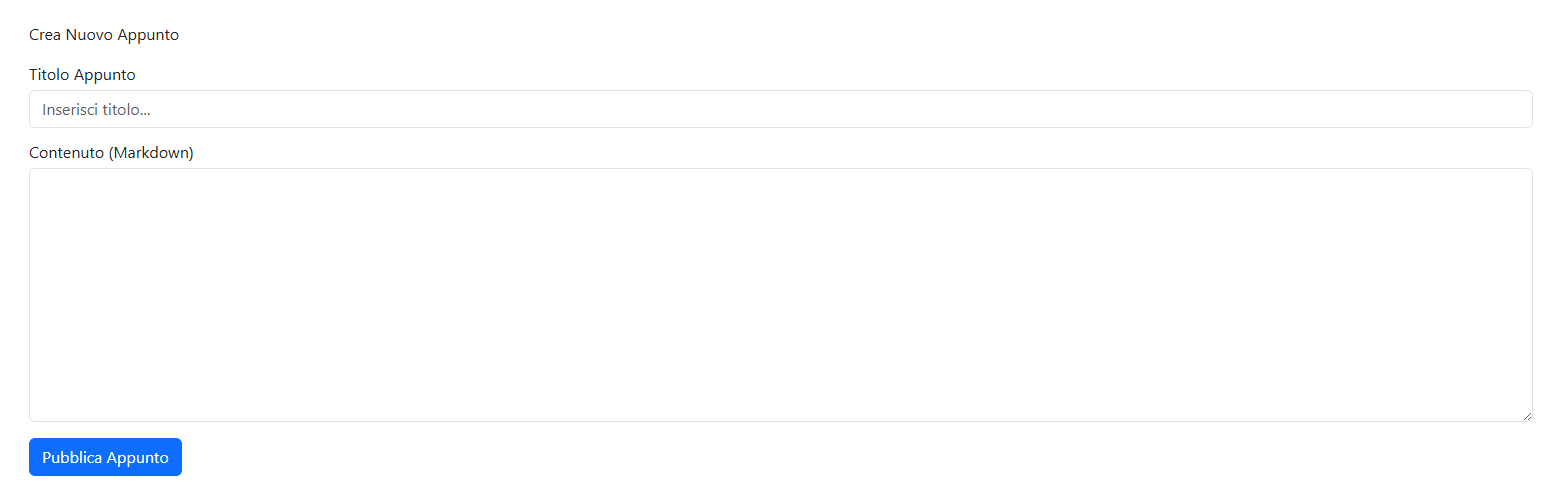
\includegraphics[width=1\textwidth]{Screen/crea_appunto.png}
    \caption{Pagina di creazione nuovo appunto}
    \label{fig:crea_appunto}
\end{figure}

\begin{figure}[H]
    \centering
    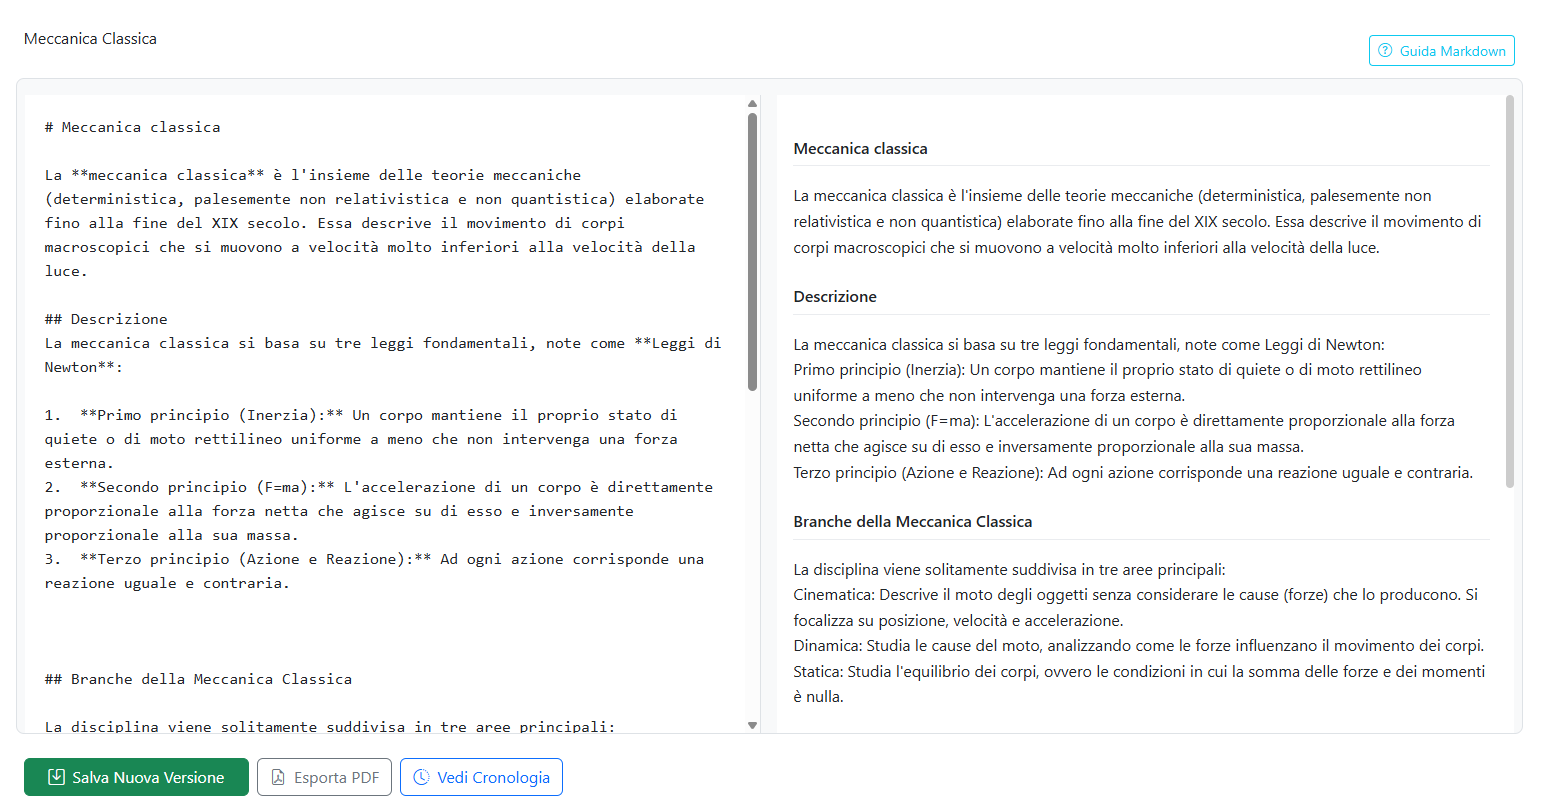
\includegraphics[width=1\textwidth]{Screen/appunto_logged.png}
    \caption{Pagina di editing appunto}
    \label{fig:appunto_logged}
\end{figure}

\section{Cronologia e Ripristino}
\noindent Per ogni appunto è disponibile la sezione \textbf{Cronologia}:
\begin{itemize}
    \item \textbf{Visualizzazione}: È possibile consultare l'elenco delle versioni passate, vedendo chi ha effettuato la modifica e quando.
    \item \textbf{Anteprima}: Selezionando \textit{``Leggi''}, l'utente può visualizzare una versione storica in sola lettura.
    \item \textbf{Ripristino}: Il tasto \textit{``Ripristina''} permette di riportare l'appunto allo stato di una versione specifica del passato. Il sistema salverà comunque lo stato attuale come una nuova versione prima del ripristino.
\end{itemize}


\begin{figure}[H]
    \centering
    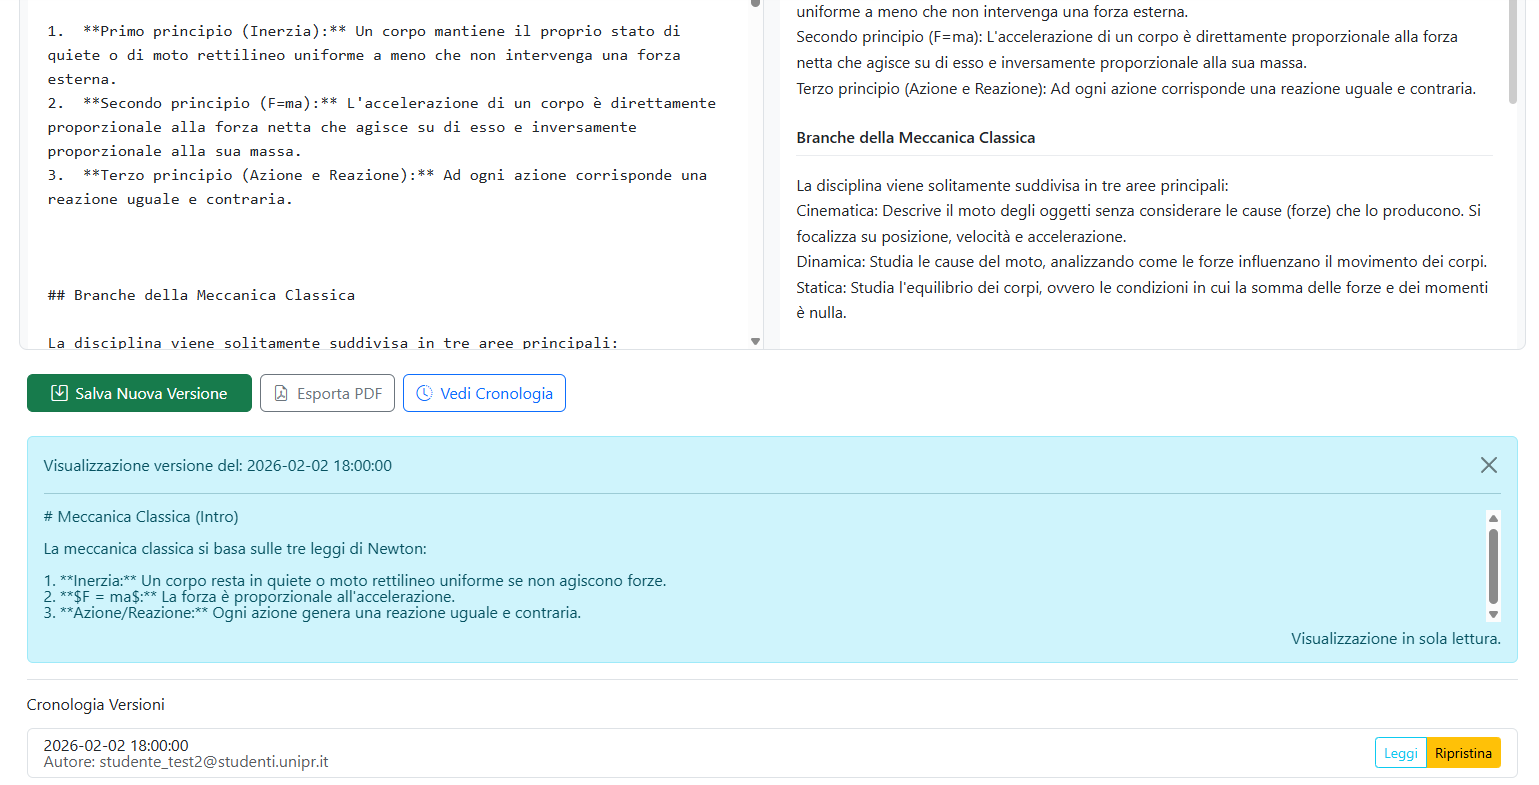
\includegraphics[width=1\textwidth]{Screen/cronologia.png}
    \caption{Cronologia}
    \label{fig:cronologia}
\end{figure}



\section{Funzionalità Extra}
\begin{itemize}
    \item \textbf{Anteprima Live}: Durante la scrittura, il sistema mostra in tempo reale come apparirà l'appunto una volta salvato.
    \item \textbf{Esportazione PDF}: Ogni appunto può essere scaricato in formato PDF per la consultazione offline.
\end{itemize}


\chapter{Modalità Amministratore}

\noindent L'utente con privilegi di \textbf{Amministratore} ha il compito di gestire l'architettura logica del Wiki e supervisionare i contenuti inseriti dagli studenti. 

\section{Accesso alla Console di Amministrazione}
\noindent Dopo aver effettuato il login con un account autorizzato (es. \texttt{admin@unipr.it}), il sistema mostra un messaggio di benvenuto specifico evidenziato in giallo (Figura \ref{fig:admin_welcome}). 
\begin{itemize}
    \item \textbf{Pulsante Gestione Catalogo}: Cliccando su questo pulsante, l'amministratore viene reindirizzato alla dashboard gestionale, dove può operare sulla struttura del sistema.
\end{itemize}

\begin{figure}[H]
    \centering
    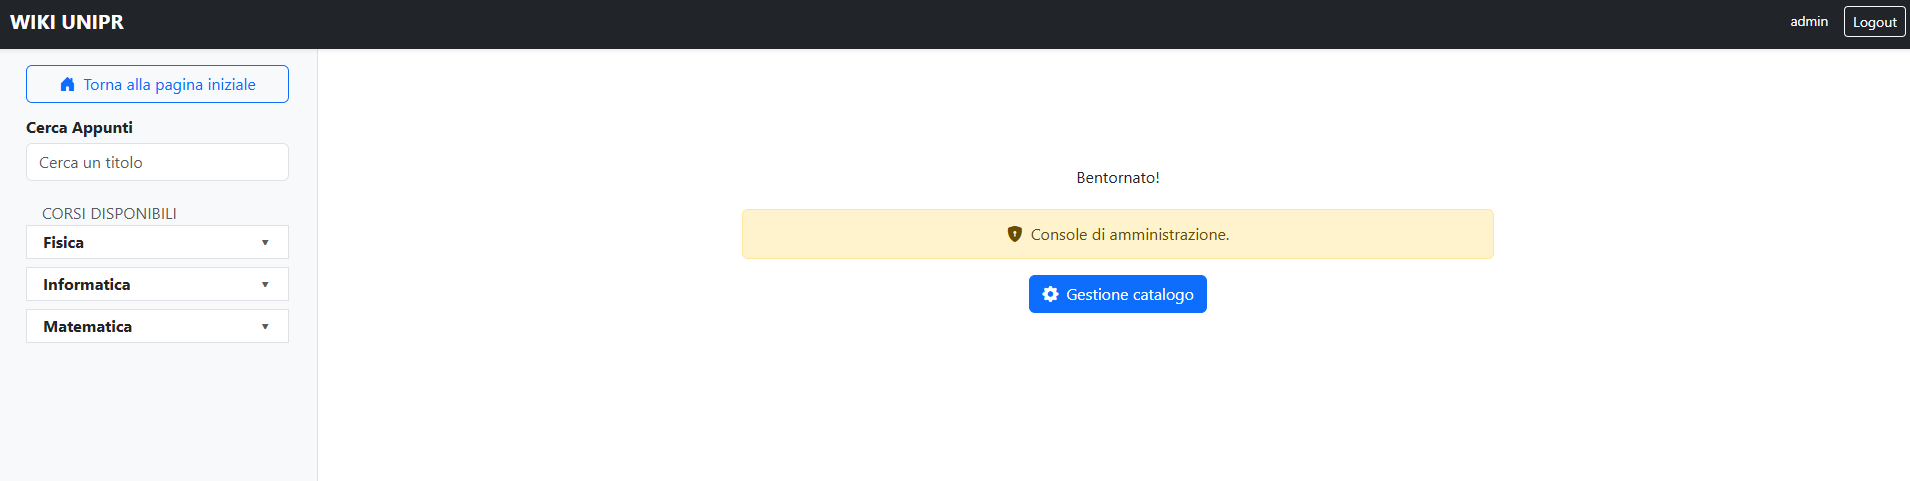
\includegraphics[width=1\textwidth]{Screen/admin_welcome.png}
    \caption{Pagina principale admin}
    \label{fig:admin_welcome}
\end{figure}

\section{Gestione della Struttura (Corsi e Argomenti)}
\noindent Tramite l'interfaccia di amministrazione, l'utente può eseguire operazioni di manutenzione strutturale (Requisito RF10):
\begin{itemize}
    \item \textbf{Corsi}: È possibile creare nuovi corsi, rinominare quelli esistenti o eliminarli(Figura \ref{fig:gest_corsi}). 
    \item \textbf{Argomenti}: Per ogni corso, l'amministratore può aggiungere, modificare o rimuovere gli argomenti(Figura \ref{fig:gest_arg}).
    \item \textbf{Cancellazione a Cascata}: L'eliminazione di un corso o di un argomento è un'operazione distruttiva che comporta la rimozione automatica di tutti gli appunti e delle relative versioni collegate.
\end{itemize}


\begin{figure}[H]
    \centering
    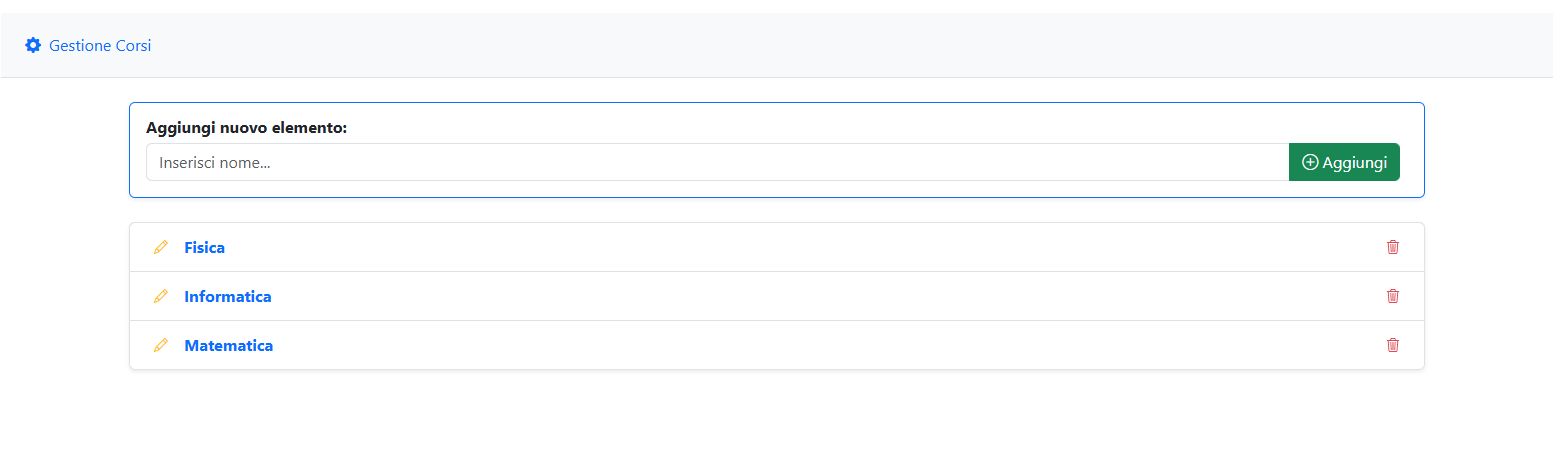
\includegraphics[width=1\textwidth]{Screen/gest_corsi.png}
    \caption{Moderazione corsi}
    \label{fig:gest_corsi}
\end{figure}


\begin{figure}[H]
    \centering
    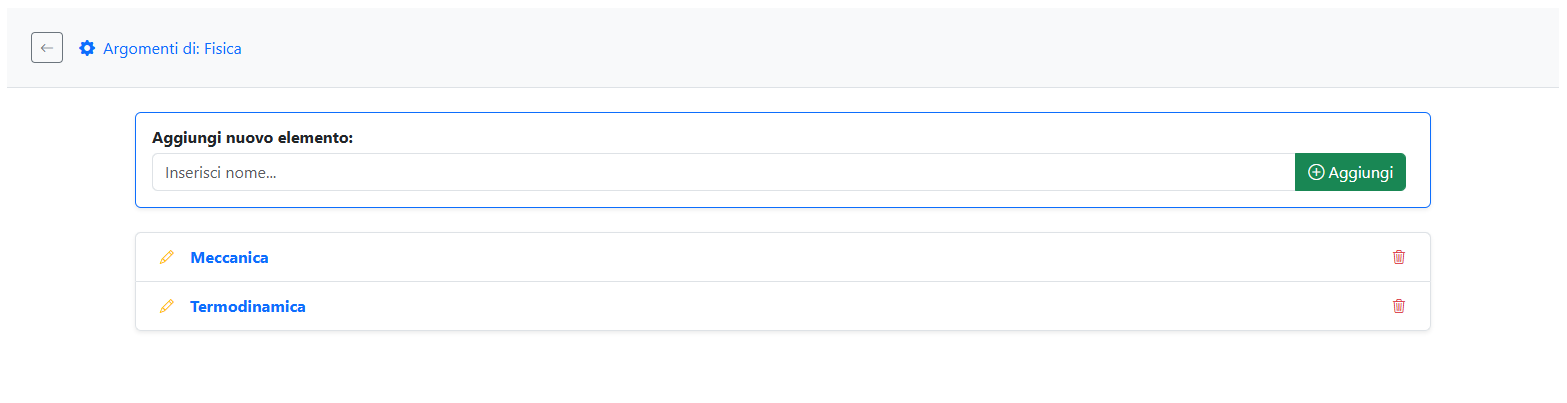
\includegraphics[width=1\textwidth]{Screen/gest_arg.png}
    \caption{Moderazione argomenti}
    \label{fig:gest_arg}
\end{figure}


\section{Moderazione degli Appunti}
\noindent A differenza dello Studente, l'Amministratore possiede poteri di moderazione sgli appunti ad esclusione della creazione:
\begin{itemize}
    \item \textbf{Modifica Titoli}: Può correggere o rinominare i titoli degli appunti per garantirne la coerenza semantica.
    \item \textbf{Eliminazione Contenuti}: È l'unico ruolo abilitato alla cancellazione definitiva di un appunto dal sistema.
\end{itemize}


\begin{figure}[H]
    \centering
    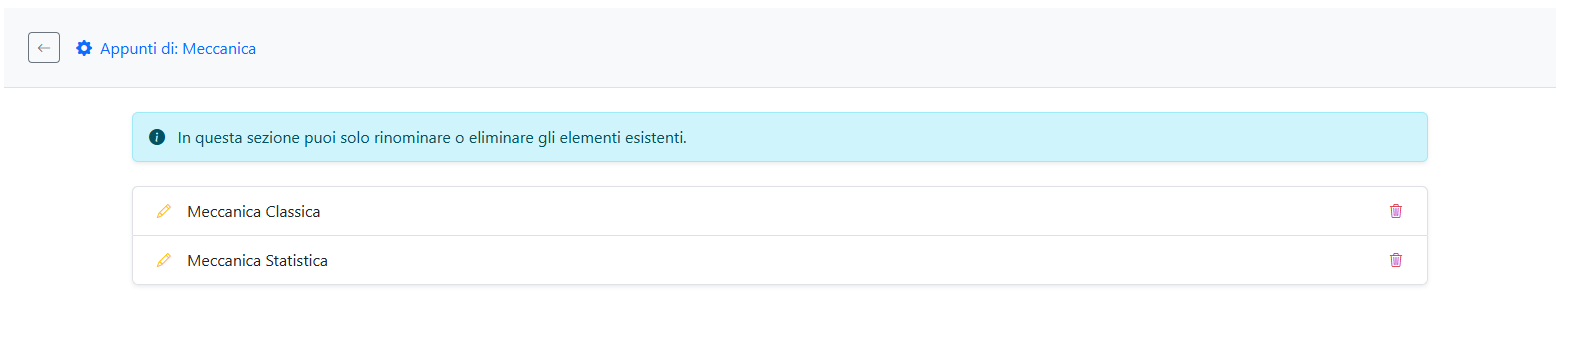
\includegraphics[width=1\textwidth]{Screen/gest_app.png}
    \caption{Moderazione appunti}
    \label{fig:gest_app}
\end{figure}

\end{document}
